\documentclass[tikz,border=4pt]{standalone}
\usepackage{amsmath,amssymb,bm}
\usepackage[T1]{fontenc}
\usepackage{newtxtext,newtxmath}
\usepackage{microtype}
\usepackage{tikz}
\usetikzlibrary{arrows.meta,positioning,calc,fit,backgrounds}

\definecolor{headLine} {HTML}{172033}
\definecolor{ink}      {HTML}{172033}
\definecolor{mutedInk} {HTML}{6B7280}
\definecolor{greyLine} {HTML}{9CA3AF}
\definecolor{greyFill} {HTML}{EEF0F3}
\definecolor{qkC}      {HTML}{D97706}
\definecolor{qkFill}   {HTML}{FEF3E2}
\definecolor{ovC}      {HTML}{7C3AED}
\definecolor{ovFill}   {HTML}{F1ECFD}
\definecolor{saeC}     {HTML}{166534}
\definecolor{saeFill}  {HTML}{CDE8D4}
\definecolor{steerC}   {HTML}{2E7D32}
\definecolor{steerFill}{HTML}{EAF6EA}
\definecolor{lambdaC}  {HTML}{D9468F}
\definecolor{lambdaFill}{HTML}{FCE7F3}
\definecolor{muC}      {HTML}{2F9E44}
\definecolor{muFill}   {HTML}{E6F8EA}
\definecolor{nuC}      {HTML}{1D4ED8}
\definecolor{nuFill}   {HTML}{DBEAFE}

\tikzset{
  >={Latex[length=2.5mm,width=1.8mm]},
  every node/.append style={line join=round},
  attnBox/.style={draw=none,fill=none,inner sep=6mm},
  nodeQK/.style={draw=qkC,line width=0.85pt,rounded corners=2.2pt,
                 fill=qkFill,font=\normalsize\bfseries,text=qkC,
                 inner sep=3pt,minimum height=6mm,minimum width=14mm,align=center},
  nodeOV/.style={draw=ovC,line width=0.85pt,rounded corners=2.2pt,
                 fill=ovFill,font=\normalsize\bfseries,text=ovC,
                 inner sep=3pt,minimum height=6mm,minimum width=14mm,align=center},
  qkflow/.style={->,line width=0.9pt,qkC,line cap=round},
  ovflow/.style={->,line width=0.9pt,ovC,line cap=round},
  qkline/.style={line width=0.95pt,qkC,line cap=round},
  ovline/.style={line width=0.95pt,ovC,line cap=round},
  saeBox/.style={draw=saeC,line width=0.95pt,rounded corners=4pt,
                 fill=saeFill,inner sep=3mm},
  feat/.style={draw=saeC!62,line width=0.45pt,fill=white,
               minimum width=5mm,minimum height=5mm,inner sep=0pt,
               font=\scriptsize\bfseries},
  featLambda/.style={draw=lambdaC,line width=1.15pt,fill=lambdaFill,
                 minimum width=5mm,minimum height=5mm,inner sep=0pt,
                 font=\small\bfseries,text=lambdaC},
  featMu/.style={draw=muC,line width=1.15pt,fill=muFill,
                 minimum width=5mm,minimum height=5mm,inner sep=0pt,
                 font=\small\bfseries,text=muC},
  featNu/.style={draw=nuC,line width=1.15pt,fill=nuFill,
                 minimum width=5mm,minimum height=5mm,inner sep=0pt,
                 font=\small\bfseries,text=nuC},
  steerPlus/.style={draw=steerC,line width=1.0pt,fill=steerFill,
                 circle,inner sep=0pt,minimum size=4.6mm,
                 font=\small\bfseries,text=steerC},
  steerArrow/.style={->,line width=1.0pt,steerC,line cap=round},
  lambdaInjArrow/.style={->,line width=0.9pt,lambdaC,line cap=round},
  muInjArrow/.style={->,line width=0.9pt,muC,line cap=round},
  nuInjArrow/.style={->,line width=0.9pt,nuC,line cap=round},
  lambdaTrace/.style={line width=0.9pt,lambdaC,line cap=round},
  muTrace/.style={line width=0.9pt,muC,line cap=round},
  nuTrace/.style={line width=0.9pt,nuC,line cap=round},
}

\begin{document}
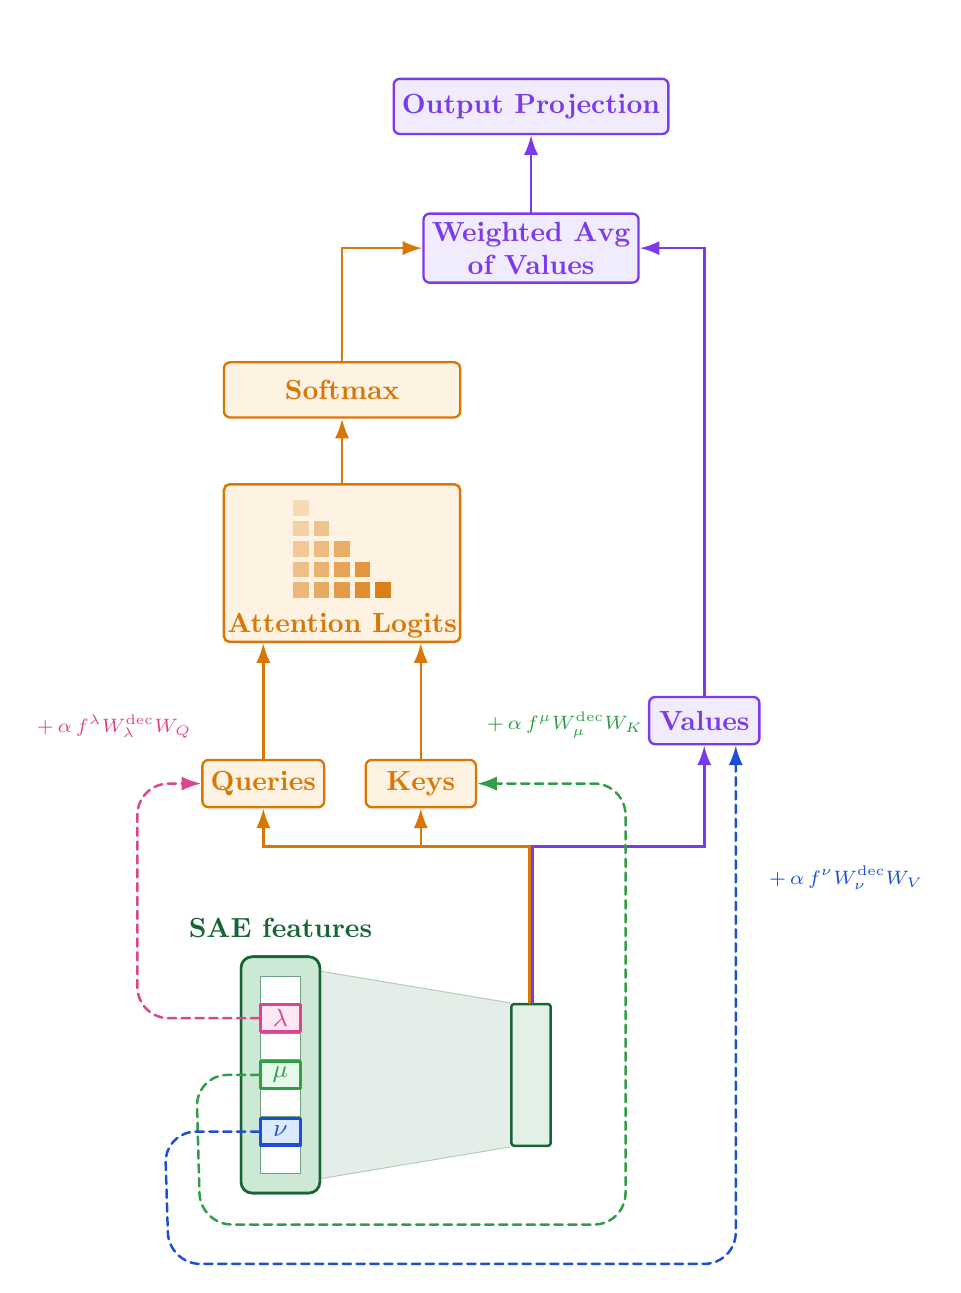
\begin{tikzpicture}[x=1mm,y=1mm]

% Attention head: same layout as attribution version.
\node[nodeQK] (queries) at (-22,34) {Queries};
\node[nodeQK] (keys)    at (-2,34)  {Keys};
\node[nodeOV] (values)  at (34,42)  {Values};

\node[draw=qkC,line width=0.9pt,rounded corners=2pt,fill=qkFill,
      minimum width=30mm,minimum height=20mm,inner sep=1mm]
      (logits) at (-12,62) {};
\node[font=\normalsize\bfseries,qkC,anchor=south,inner sep=1pt]
  at ([yshift=0.3mm]logits.south) {Attention Logits};

\pgfmathsetmacro{\HC}{2.6}
\foreach \r in {0,...,4} {%
  \foreach \c in {0,...,4} {%
    \pgfmathtruncatemacro{\active}{\c <= \r ? 1 : 0}%
    \pgfmathsetmacro{\op}{\active * (0.20 + 0.18*\c + 0.07*(\r-\c))}%
    \pgfmathsetmacro{\xc}{(\c-2)*\HC}%
    \pgfmathsetmacro{\yc}{1.8 + (2-\r)*\HC}%
    \fill[qkC,opacity=\op]
      ([xshift=\xc mm-1mm,yshift=\yc mm-1mm]logits.center)
      rectangle
      ([xshift=\xc mm+1mm,yshift=\yc mm+1mm]logits.center);
  }%
}

\node[nodeQK,minimum width=30mm,minimum height=7mm]
      (softmax) at (-12,84) {Softmax};
\node[nodeOV] (wavg) at (12,102) {Weighted Avg\\ of Values};
\node[nodeOV,minimum width=30mm,minimum height=7mm]
      (oproj) at (12,120) {Output Projection};

\coordinate (jx) at (12,26);
\coordinate (jxQK) at ([xshift=-0.18mm]jx);
\coordinate (jxOV) at ([xshift=0.18mm]jx);
\draw[qkflow] (jxQK) -| (keys.south);
\draw[qkflow] (jxQK) -| (queries.south);
\draw[ovflow] (jxOV) -| (values.south);

\draw[qkflow] (keys.north)    -- (keys.north    |- logits.south);
\draw[qkflow] (queries.north) -- (queries.north |- logits.south);
\draw[qkflow] (logits.north) -- (softmax.south);
\draw[qkflow] (softmax.north) -- ++(0,3) |- (wavg.west);
\draw[ovflow] (values.north) |- (wavg.east);
\draw[ovflow] (wavg.north) -- (oproj.south);

\coordinate (xTop) at (12,16);
\coordinate (outTop) at (54,124);
\begin{scope}[on background layer]
  \node[attnBox,fit=(keys)(values)(logits)(softmax)(wavg)(oproj)(xTop)(outTop)] (head) {};
\end{scope}

% Activation block + SAE with three features that drive interventions.
\node[draw=saeC,line width=0.9pt,rounded corners=1pt,fill=saeFill!60,
      minimum width=5mm,minimum height=18mm,inner sep=0pt]
      (postLNvec) at (12,-3) {};

\draw[qkline]
  ([xshift=-0.18mm]postLNvec.north) -- (jxQK) -- (keys.south |- jx);
\draw[ovline]
  ([xshift=0.18mm]postLNvec.north) -- (jxOV) -- (values.south |- jx);

\node[saeBox,minimum width=10mm,minimum height=30mm,
      left=24mm of postLNvec.west,anchor=east] (sae) {};

\begin{scope}[on background layer]
  \fill[saeC!38,opacity=0.30]
    (postLNvec.north west) -- ([yshift=-2mm]sae.north east) --
    ([yshift=2mm]sae.south east) -- (postLNvec.south west) -- cycle;
  \draw[saeC!55,opacity=0.55,line width=0.35pt]
    (postLNvec.north west) -- ([yshift=-2mm]sae.north east);
  \draw[saeC!55,opacity=0.55,line width=0.35pt]
    (postLNvec.south west) -- ([yshift=2mm]sae.south east);
\end{scope}

\node[saeBox,minimum width=10mm,minimum height=30mm,
      left=24mm of postLNvec.west,anchor=east] (sae) {};

\foreach \i in {1,...,7} {
  \node[feat,minimum width=5mm,minimum height=3.4mm]
        (f\i) at ([yshift={(\i-4)*3.6mm}]sae.center) {};
}
\node[featLambda,minimum height=3.4mm] (flam) at (f6.center) {$\lambda$};
\node[featMu,minimum height=3.4mm]     (fmu)  at (f4.center) {$\mu$};
\node[featNu,minimum height=3.4mm]     (fnu)  at (f2.center) {$\nu$};

\node[font=\normalsize\bfseries,saeC,align=center,above=1mm of sae.north,anchor=south]
  {SAE features};

% Routes from SAE features to the corresponding intervention sites.
% Lambda -> Queries: out left, up to queries level, then right into queries.west.
\draw[lambdaTrace,densely dashed,->,rounded corners=4mm]
  (flam.west) -| (-38,34) -- (queries.west);

% Mu -> Keys: route around the bottom and up to keys.east (stays below SAE box).
\draw[muTrace,densely dashed,->,rounded corners=4mm]
  (fmu.west) -- ([xshift=-8mm]fmu.west)
  -- (-30,-22)
  -- (24,-22)
  -- (24,34)
  -- (keys.east);

% Nu -> Values: route along the bottom, then straight UP into the bottom of Values.
\draw[nuTrace,densely dashed,->,rounded corners=4mm]
  (fnu.west) -- ([xshift=-12mm]fnu.west)
  -- (-34,-27)
  -- (38,-27)
  -- ([xshift=4mm]values.south);

% Labels: "+" prefix in the feature colour, sitting above the relevant box.
\node[font=\scriptsize\bfseries,text=lambdaC,anchor=south east]
  at ([yshift=1.4mm]queries.north west) {$+\,\alpha\,f^{\lambda} W^{\mathrm{dec}}_{\lambda} W_Q$};
\node[font=\scriptsize\bfseries,text=muC,anchor=south west]
  at ([yshift=1.4mm]keys.north east) {$+\,\alpha\,f^{\mu} W^{\mathrm{dec}}_{\mu} W_K$};
\node[font=\scriptsize\bfseries,text=nuC,anchor=west]
  at (41,22) {$+\,\alpha\,f^{\nu} W^{\mathrm{dec}}_{\nu} W_V$};

\end{tikzpicture}
\end{document}
